\documentclass{article}
\usepackage{graphicx}
\usepackage{amsmath}
\usepackage{amssymb}
\usepackage{amsfonts}
\usepackage{amsthm}
\usepackage{subcaption}
%\usepackage{subfigure}
\graphicspath{ {plots/} }

\newtheorem{thm}{Theorem}[section]
\newtheorem{cor}[thm]{Corollary}
\newtheorem{lem}[thm]{Lemma}
\newcommand{\pdiv}[2]{{\frac{\partial#1}{\partial#2}}}

\title{Kelly's Criterion}
\date{2021-09-01}
\author{Eldad Kronfeld}


\begin{document}
	\maketitle
	\thanks{Thank you, Hagai for the continuing patience and support along the way.}
	\tableofcontents
	\newpage
	\begin{abstract}
		This is a paper about the mathematical model proposed by John Kelly at the early 1950s, 
		however instead of looking at the model from the lenses of games and gambles, each of our gamble is an option we can invest in until the next round of the model, at the beginning I will explain the basic concept behind the model and show simple example for one investments with multiple outcomes at each round, the results will be shown by using Monte Carlo simulation, later on I will expend the module to include multiple investments each with multiple outcomes.
	\end{abstract}
	\section{The Base model}
	Kelly's Criterion is an infinite model in discrete time frames, which I will call ticks$\backslash$rounds.
	at each round we have sum of money that we would like to invest and the model represent what happens each round with the split that we decided on.\newline
	However, the premise of the model is that the investments or gambles we take each round have expectations that are greater then 1,
	$$\textbf{E}_{gain} \ge 1$$
	meaning that in the long run we can expect that we will yield revenue from the venture and not loss from it.
	\newline
	\textbf{Note:} through all of the explanations and simulations I will normalize the odds to be such as that we start with 1$\textdollar$ and each gain will be noted as $\gamma\cdot F_{N-1}$, where $F_{N-1}$ denotes the sum of money from round $N-1$ and $\gamma$ denotes the gain and $\gamma\in[0,\infty)$, so when $\gamma = 1$ it means that there is no gain and no loss at all, however when 
	$\gamma > 1$ we gain money and when $ 0\le \gamma < 1$ we can expect to loss money.
	\newline\newline
	if we try to define a simple model, where we have 1 investment with $k$ outcomes, where each outcome have $p_i$ probability of happening and we invest $f$ amount of money and keep $b=1-f$ 
		\begin{equation}
			\label{nes}
			F_N = \Bigg\{
			\begin{aligned}
				&(b + f\cdot \gamma _i)F_{N-1} &&for\enspace i=1,..,k \\
				&1 &&for \enspace i=0
			\end{aligned}
		\end{equation}
	\\
	this equation represent that if outcome $i$ happens then the part that we didn't invest in $(1-f)$ doesn't change, however the part that we did invest $f$ changes by $\gamma_i$.
	\newline
	ultimately the way I looked at it, which helped me later to define more complicated model would be:\newline
	\textit{let} $X$ be random variable that represent the gain of each outcome, then if the outcome is $\gamma_i$ then $P(X=\gamma_i) = p_i$, this will help us look at the exponential growth and develop a way to find the optimal fraction $f$ in each round to achieve the optimal returns.
	\\
	now let's look for the fraction \(f\) that produces the best gain, because equation \ref{nes} we can deduce that the growth rate from an investment is exponential , then:
	\begin{equation}
		\label{exp:FN}
		F_N = F_0e^{G_{N}N}
	\end{equation}
	so \(G_N = \frac{1}{N}log(\frac{F_N}{F_0}) = \sum_{i=1}^{k} \frac{W_i}{N}log(b + \gamma_i f)\), however when we take N to \(\infty\) in equation \ref{exp:FN} we get the following equation:
	\begin{equation}
		\label{gain:func1}
		G = \lim_{N \to \infty} \sum_{i=1}^{k} \frac{W_i}{N}log(b+\gamma_i f) = \sum_{i=1}^{k} p_i log(b+\gamma_i f)
	\end{equation}
	then we would like to look for the maximum.
	\newline \newline
	\begin{thm}\label{thm1}
		$f(x) = -log(b(x)+\gamma x)$ is convex when $x\in (0,\infty)$.
	\end{thm}
	\begin{proof}
		$\pdiv{f}{x} = -\frac{\gamma - 1}{b+\gamma x}$ and the second derivative is 
		$\frac{\partial f}{\partial x^2} = \frac{(\gamma -1) ^2}{(b+\gamma x)^2}$\\
		second derivative is always positive, then $f(x)$ is convex.
		\newline
	\end{proof}
	
	\begin{lem}
		\(G(f) = \sum_{i=1}^{k} p_i log(b+\gamma_i f)\) is concave.
	\end{lem}
	\begin{proof}
		when we look at equation \ref{gain:func1} as a function of $f$,\\
		$G(f)$ is concave $\iff$ $-G(f)$ is convex.
		\[-G(f) = \sum_{i=1}^{k} p_i (-log(b+\gamma_i f))\]
		however a positive weighted sum of convex functions, is a convex function, each component $s_i = p_i log(b+\gamma_i f)$ is convex because $\gamma _i$ is non-negative , and $0\le p_i \le 1$ and Theorem \ref{thm1} ,then \(-G(f)\) is convex, making $G(f)$ concave.
		\newline
	\end{proof}

	because $G$ is concave, we will be able to find it's maximum by calculating the root of the Derivative, which is 
	\[\pdiv{G}{f} = \sum_{i=0}^{k} p_i \frac{\gamma_i - 1}{b+\gamma_i f} = 0\] 
	and we know that such a root exist inside $[0,1]$ because of last lemma, stating that $G(f)$ is concave making it's second derivative always non-positive, then the maximum point should be either at the end of the range at 1 or somewhere inside it, because $G'(0) = \sum_{i=0}^{k} p_i \frac{\gamma_i - 1}{b} = \frac{1}{b}(E_{gain} - \sum_{i = 1}^{k} p_i) = \frac{1}{b}(E_{gain} - 1) > 0$, this statement is true because the sum of all the possibilities is $1$ and $E_{gain} \ge 1$.
	\newline
	the actual root is very tough to find, however at my own python implementation I used Brent's method which is a hybrid method combining bisection method, the secant method and inverse quadratic interpolation, which was highly recommended by Scipy's optimization documentation.
	\newline
	\section{First Model's Monte Carlo Simulations}
	After looking at the model analytically and arguing that an optimal fraction does exist, we can simulate scenarios that will help us validate our statements.\\
	In order to accomplish such a task, I wrote code in point that represent a simulation, where in each round of the simulation we will pick one of the outcomes, however the probability to pick a certain outcome will be defined, so less common occurrences will be less likely to happen then the more common ones.\\
	After creating classes in order to define the probabilities and the general flow of the simulation I saved for each instance of the simulation I ran, the amount of fortune at each round in order to plot graphs like Fig \ref{Fig:single1} in order to show that our calculation were right and the optimal value does exist and it works in real life situations.\\
	\begin{figure}[h]
		\begin{subfigure}{0.525\textwidth}
			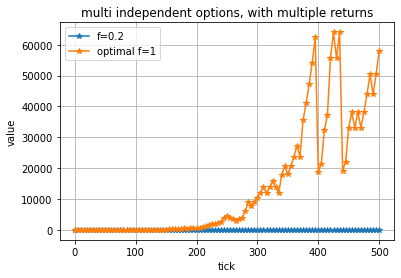
\includegraphics[width=0.9\linewidth]{single1} 
			\label{fig:subim1}
		\end{subfigure}
		\begin{subfigure}{0.525\textwidth}
			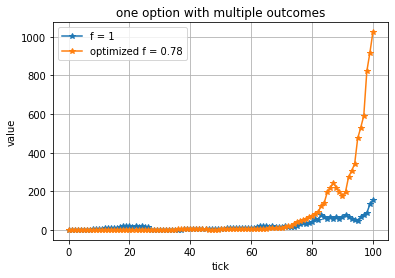
\includegraphics[width=0.9\linewidth]{single2}
			\label{fig:subim2}
		\end{subfigure}
		\caption{Two random simulation with and without optimal value}
		\label{Fig:single1}
	\end{figure}	
	
\end{document}